\chapter{Das Registrierungsformular}

Der wohl komplizierteste Teil dieser Diplomarbeit ist der Aufbau und die korrekte Validierung des Registrierungsformulars. Das Ziel ist den Benutzern eine möglichst einfache und schnelle Registrierung, unter Berücksichtigung des derzeitigen Standorts und der dazugehörigen Benutzergruppe, anzubieten. Dafür wurde ein Algorithmus entwickelt, welcher bei der \texttt{ngAfterViewInit} Lifecycle-Hook-Methode im \texttt{UserprofileComponent} seinen Start nimmt.

\section{Der Algorithmus hinter dem dynamischen Aufbau}

\begin{figure}[H]
	\centerline{
		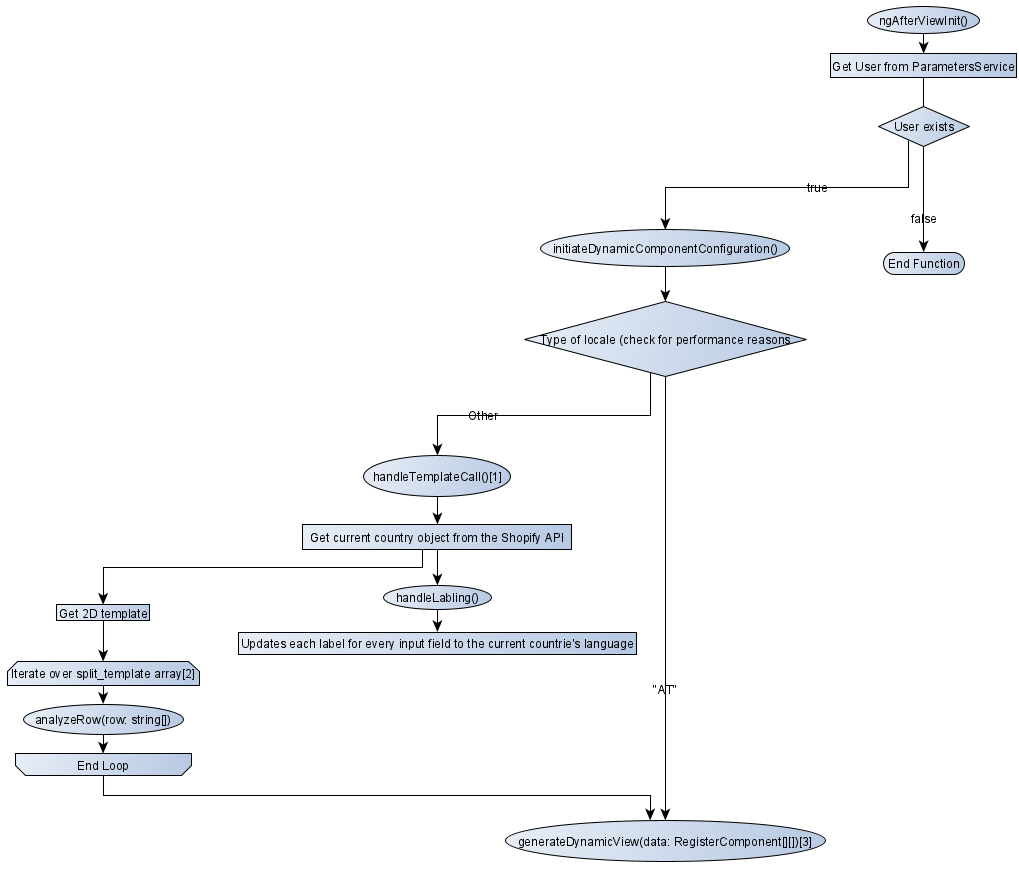
\includegraphics[width=1\textwidth, frame]{./grafiken/RF_Flussdiagramm.png}
	}
	\vskip0pt
	\caption{Flussdiagramm des Algorithmus}
	\label{fig:fc}
\end{figure}

\subsection{\texttt{initiateDynamicComponentConfiguration()}}

Wenn das User-Objekt, welches von der Backend API abgefragt und erfolgreich als globale Objekt variable gespeichert wurde, wird die \texttt{initiateDynamicComponentConfigu\\ration()}-Methode aufgerufen. Aus Performance-Gründen basiert die nächste Überprüfung auf den Wert der aktuellen Lokale. Gleicht dieser den Wert "AT", so wird ein vorgefertigtes Template für ein österreichisches RF, dargestellt im Listing~\ref{lst:template_form_aut}, für die Weiterverwendung benützt. Da davon ausgegangen wird, dass sich vor allem in der Anfangsphase nach der Veröffentlichung hauptsächlich österreichische Kunden ein Konto erstellen, spart dieser Weg enorm viel Zeit, da sofort mit der Erstellung des RF begonnen werden kann.

\begin{lstlisting}[caption={Vordefiniertes Template für das RF},captionpos=b, language=JavaScript,label={lst:template_form_aut}]
export const AUSTRIAN_PRIVATE_PERSON_FORM_Template = [
	[{ type: GenderComponent }],
	[
		{ type: FirstnameComponent, options: { label: "Vorname" } },
		{ type: LastnameComponent, options: { label: "Nachname" } },
	],
	[{ type: StreetComponent, options: { label: "Straße und Hausnummer" } }],
	[
		{ type: CityComponent, options: { label: "Stadt" } },
		{ type: PostalcodeComponent, options: { label: "Postleitzahl" } },
	],
	[
	{
		type: PhoneComponent,
		options: { label: "Telefonnummer", phonePrefix: 43 },
	},
	{ type: DateofbirthComponent },
	],
];
\end{lstlisting}

\subsection{\texttt{handleTemplateCall()}}

Anderenfalls wird als nächster Schritt die \texttt{handleTemplateCall()}-Methode aufgerufen, markiert im Flussdiagramm~\ref{fig:fc} mit [1], welche, basierend auf den Wert der aktuellen Lokale, auf die Shopify API zugreift, um ein \texttt{Country}-Objekt abzurufen. Wurde diese Operation beendet folgt ein Update auf eine Map, welche vorläufig die Labels für die Wrapper-Objekte speichert. Nach dem das Template geladen wurde, wird über jedes einzelne Element iteriert, markiert im Flussdiagramm~\ref{fig:fc} mit [2], um daraus eine oder mehrere Zeilen zu generieren. Anschließend werden diese in ein 2D Array gespeichert, welches dann der \texttt{generateDynamicView()}-Methode zu Generierung des RF übergeben wird. 

\subsection{\texttt{analyzeRow()}}

\begin{lstlisting}[caption={Erstellung des 2D Arrays für den Aufbau des RF},captionpos=b, language=JavaScript,label={lst:analyzeRow}]
private analyzeRow(row: string[]): RegisterComponent[][] {
	let addGenderC = false;
	let result: RegisterComponent[][] = [];
	let componentRow: RegisterComponent[] = [];
	
	for (let i = 0; i < row.length; i++) {
		let rowEl = row[i];
		
		if (!addGenderC) {
			if (rowEl.includes("firstName") || rowEl.includes("lastName")) {
				let genderComponent: RegisterComponent[] = [
				{ type: GenderComponent },
				];
				result.push(genderComponent);
				addGenderC = true;
			}
		}
		
		if (rowEl.includes("company") && this.user.isPrivatePerson) {
			break;
		}
		
		for (const x of this.valueMap.keys()) {
			if (rowEl.includes(x)) {
				let compEl: RegisterComponent = {
					type: this.valueMap.get(x),
				};
				
				if (
				compEl.type.prototype ===
				ZoneComponent.prototype
				) {
					compEl.options.zones = this.countryFromService.zones.map(
					(x) => x.name
					);
					this.user.zone = compEl.options.zones[0];
				}
				
				if (
				compEl.type.prototype ===
				PhoneComponent.prototype
				) {
					compEl.options.phonePrefix = this.countryFromService.phoneNumberPrefix;
				}
				
				if (this.labels.get(x)) {
					compEl.options.label = this.labels.get(x);
				}
				
				componentRow.push(compEl);
				if (rowEl.includes("phone")) {
					let dateofbirthComponent: RegisterComponent = {
						type: DateofbirthComponent,
					};
					componentRow.push(dateofbirthComponent);
				}
				break;
			}
		}
	}
	result.push(componentRow);
	return result;
}
\end{lstlisting}

Die im Listing~\ref{lst:analyzeRow} beschriebene \texttt{analyzeRow()}-Methode nimmt ein Array von Zeichenfolgen als Parameter und gibt ein 2D-Array von \texttt{RegisterComponent}-Wrapper-Objekten zurück. Obwohl nur eine Reihe aus dem Template, also z. B. \texttt{[\{firstName\} \{lastname\}]}, überprüft wird, kann es wie in diesem Fall sein, dass ein Input zusätzlich darüber erzeugt werden muss. So wird in Zeile 9 überprüft, ob der \texttt{GenderComponent} schon hinzugefügt wurde. Trifft das und die Überprüfung, ob in diesem Durchgang der \texttt{FirstnameComponent} und der \texttt{LastnameComponent} erzeugt werden, wird der \texttt{GenderComponent} als erster eingefügt. Dieser ist für die Auswahl der Anrede zuständig. Der selbe Mechanismus kann auch in Zeile 51 gefunden werden, wo es nötig ist, den \texttt{DateofbirthComponent}, welcher für die Eingabe des Geburtstages verantwortlich ist, neben den \texttt{PhoneComponent} zu generieren.

Anschließend wird in Zeile 19 sicher gestellt, dass eine Privatperson keine Auswahl einer Firma präsentiert wird.

Um nun tatsächlich aus dem Template Objekte zu erzeugen, wird ab Zeile 23 über Schlüssel einer Map, beschrieben im Listing~\ref{lst:valueMap}, welche den String eines Templates als \texttt{key} und den korrespondierenden Objekten als \texttt{value} hat, iteriert. 

\begin{lstlisting}[caption={valueMap in der \texttt{analyzeRow()}-Methode},captionpos=b, language=JavaScript,label={lst:valueMap}]
export class ValueMapper {
	static COMPONENT_VALUE_MAP: Map<string, Type<any>> = new Map();
	
	static COMPONENT_VALUE_MAPPER(){
		this.COMPONENT_VALUE_MAP.set('firstname', FirstnameComponent);
		this.COMPONENT_VALUE_MAP.set('lastname', LastnameComponent);
		this.COMPONENT_VALUE_MAP.set('company', BusinessNameComponent);
		this.COMPONENT_VALUE_MAP.set('address1', StreetComponent);
		this.COMPONENT_VALUE_MAP.set('zip', PostalcodeComponent);
		this.COMPONENT_VALUE_MAP.set('city', CityComponent);
		this.COMPONENT_VALUE_MAP.set('phone', PhoneComponent);
		this.COMPONENT_VALUE_MAP.set('dateOfBirth', DateofbirthComponent);
		this.COMPONENT_VALUE_MAP.set('gender', GenderComponent);
		this.COMPONENT_VALUE_MAP.set('zone', ZoneComponent);
		this.COMPONENT_VALUE_MAP.set('province', ZoneComponent);
		this.COMPONENT_VALUE_MAP.set('state', ZoneComponent);
		return ValueMapper.COMPONENT_VALUE_MAP;
	}
}
\end{lstlisting}

Im ersten Schritt wird, wenn das vom Template angeforderte Feld in der Map existiert, das Wrapper-Objekt erzeugt. 

Wenn dieses den Typ \texttt{ZoneComponent} besitzt, handelt es sich um ein RF, welches für ein Land wie Italien oder Amerika bestimmt ist. Um eine erfolgreiche Registrierung in diesen Ländern abzuschließen, muss hier nämlich die zugehörige Provinz (IT) oder der zugehöriger Bundesstaat (US) angegeben werden. Natürlich funktioniert das für jedes Land, welches dieses Kriterium erfüllen muss. Diese Daten werden anschließend aus dem \texttt{Country}-Objekt der Shopify API gelesen und als \texttt{zone}-Property in die \texttt{options} gespeichert. 

Im Anschluss wird ebenfalls von diesem Objekt die Telefonnummernvorwahl in die \texttt{options} als \texttt{phoneNumberPrefix}-Property der Wrapper-Klasse gespeichert.

Als letzter Schritt in dieser Methode werden von Zeile 46 bis 48 die Labels, welche vorher in einer Map gespeichert wurden, als \texttt{label}-Property in die \texttt{option} der Wrapper-Objekt gespeichert. 

Nach dem Abschluss wird das Ergebnis an die Schleife der \texttt{initiateDynamicComponent\\Configuration()}-Methode geliefert und als Zwischenergebnis gespeichert. Wenn die Iteration fertig ist, werden die Zwischenergebnisse zusammengefasst und an die nächste Methode übergeben.

\begin{figure}[h]
	\centerline{
		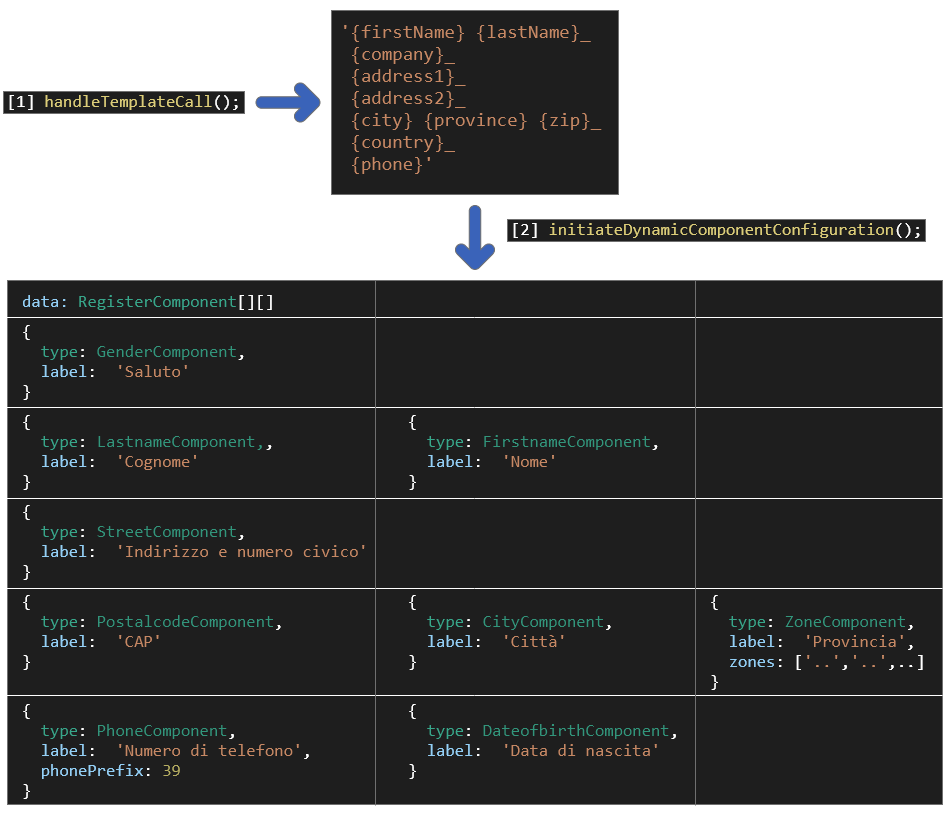
\includegraphics[width=1\textwidth, frame]{./grafiken/RF_Visualisierter Ablauf_1.png}
	}
	\vskip0pt
	\caption{Visualisierter Datenfluss vom Template bis zur Erstellung des 2D-Arrays}
\end{figure}

\subsection{\texttt{generateDynamicView(data: RegisterComponent[][])}}

\begin{lstlisting}[caption={Die \texttt{generateDynamicView()}-Methode},captionpos=b, language=JavaScript,label={lst:generateDynamicView}]
generateDynamicView(data: RegisterComponent[][]) {
for (const element of data) {
	const factory = this.componentFactoryResolver.
	resolveComponentFactory(AutoRowComponentGenerator);
	
	const ref = this.viewContainerRef.createComponent(factory);
	(<AutoRowComponentGenerator>ref.instance).data = element;
	ref.changeDetectorRef.detectChanges();
}
this.bindUserDataToViewData();
}
\end{lstlisting}

Die \texttt{generateDynamicView()}-Methode, markiert im Flussdiagramm~\ref{fig:fc} mit [3], iteriert über jedes Array, um eine \texttt{AutoRowComponentGenerator}-Klasse zu erzeugen. Aus jedem Array in dem 2D-Array wird also eine eigene Reihe für das RF erzeugt. Dabei wird die von Angular bereitgestellte \texttt{ComponentFactoryResolver}-Klasse verwendet, um aus einer Klasse einen Component zu erstellen. 
Jede Reiher, also jeder \texttt{AutoRowComponentGenerator}, wird dann nacheinander in die HTML-Datei durch eine \texttt{ViewContainerRef} eingefügt. Die \texttt{ViewContainerRef} verweist auf ein HTML-Element, wie es das Listing~\ref{lst:html} beschreibt.

\begin{lstlisting}[caption={ViewContainerRef verweist auf \#componentHook},captionpos=b, language=JavaScript,label={lst:html}]
<form #dynamicForm>
	<div #componentHook></div>
</form>
\end{lstlisting}

Das Array aus Wrapper-Klassen wird anschließend dem erzeugten Component als \texttt{data}-Objekt übergeben. \texttt{detectChanges()} sagt dem Component, dass er die Lifecycle-Hook-Methode \texttt{ngAfterViewInit()} erneut aufrufen muss. Wie gleich erklärt wird, ist diese dafür verantwortlich, dass die übergebenen Daten verarbeitet werden.

Da das Registrierungsformular in der Profilübersicht wieder verwendet wird, ist es wichtig, die Daten, welche vom Benutzer bereits vorhanden sind, in das frisch erstellte RF durch die Methode \texttt{bindUserDataToViewData()} wieder einzubinden.

\subsection{Die \texttt{AutoRowComponentGenerator}-Klasse}

\begin{lstlisting}[caption={Die \texttt{ngAfterViewInit()}-Methode der \texttt{AutoRowComponentGenerator}-Klasse},captionpos=b, language=JavaScript,label={lst:nginARCG}]
ngAfterViewInit(): void {
	for (const x of this.data) {
		const factory = this.componentFactoryResolver
		.resolveComponentFactory(x.type);
		
		const ref = this.viewContainerRef.createComponent(factory);
		this.checkComponentRef(ref, x);
		ref.changeDetectorRef.detectChanges();
	}
	this.addClasses();
}
\end{lstlisting}

Anders als bei der \texttt{generateDynamicView()}-Methode wird nicht über ein 2D-Array iteriert, um ein Array an Daten zu übergeben, sondern über das tatsächliche Array, welches eine Reihe aus Feldern repräsentiert. Diese werden dann nach der Reihe auf die selbe Weise erzeugt. \texttt{checkComponentRef()} bindet die \texttt{options} der Wrapper-Klasse an die erzeugten Components, wie im Listing~\ref{lst:ccr} gezeigt wird.

\newpage

\begin{lstlisting}[caption={Die \texttt{checkComponentRef()}-Methode der \texttt{AutoRowComponentGenerator}-Klasse},captionpos=b, language=JavaScript,label={lst:ccr}]
checkComponentRef(ref: ComponentRef<any>, component: RegisterComponent) {
	if (component.options) {
		if (component.options.zones) {
			(ref.instance as ZoneComponent).zones = component.options.zones;
		}
		
		if (component.options.label) {
			(ref.instance as ComponentValueConfigurator).setLabel(
			component.options.label
			);
		}
		
		if (component.options.phonePrefix) {
			(ref.instance as PhoneComponent).setPhonePrefix(
			component.options.phonePrefix
			);
		}
	}
}
\end{lstlisting}

Abschließend werden noch CSS-Klassen für bestimmte Komponenten vergeben.

\begin{figure}[H]
	\centerline{
		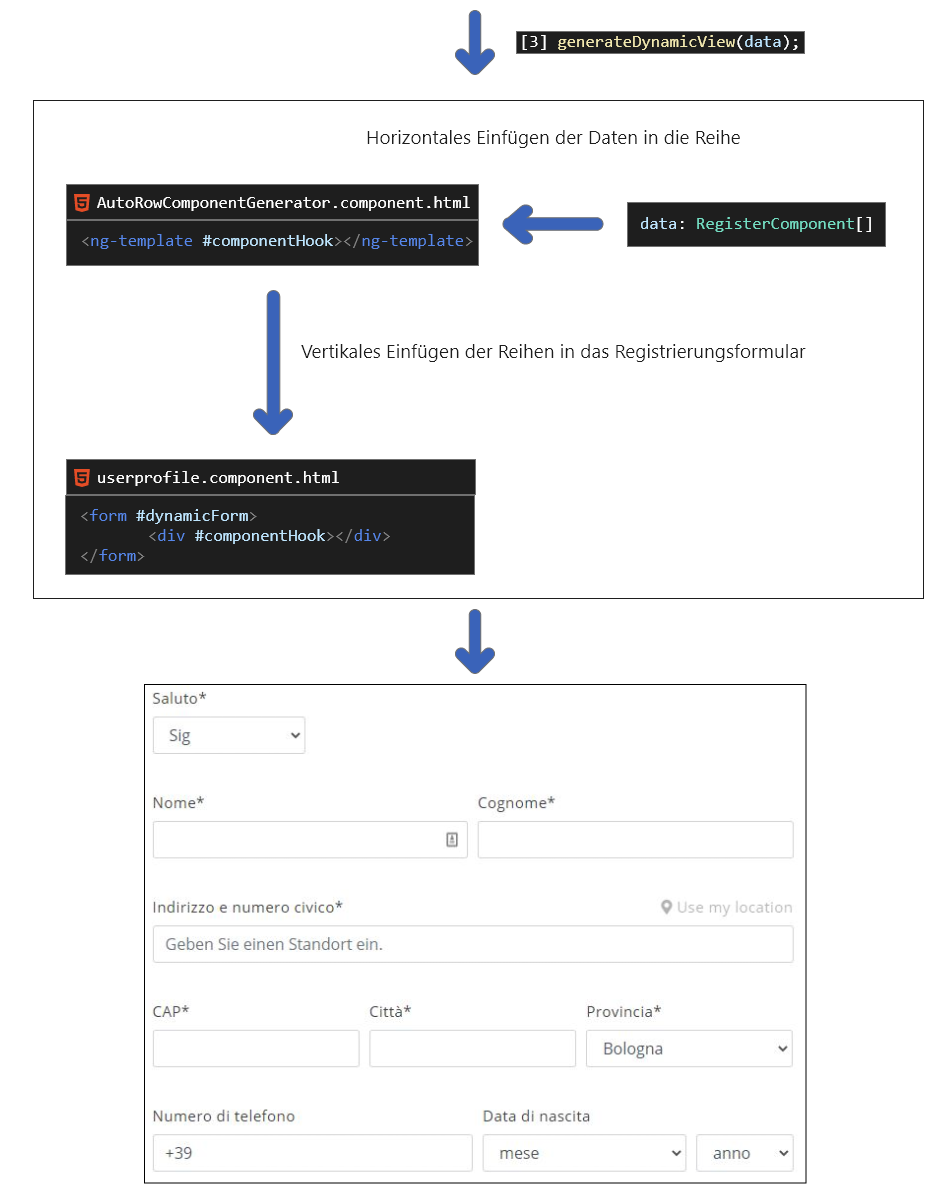
\includegraphics[width=1\textwidth, frame]{./grafiken/RF_Visualisierter Ablauf_2.png}
	}
	\vskip0pt
	\caption{Visualisierter Datenfluss vom 2D-Array bis zum fertigen RF}
\end{figure}

\section{Die Validierungsmethodik}

\section{Die Komfortfunktionen}



